\chapter{Documento de Requisitos}\label{cap:06requisitos}

Este capítulo se divide en cuatro secciones: \ref{sec:06intro} Introducción, \ref{sec:06rf} Requisitos funcionales, \ref{sec:06rnf} Requisitos no funcionales y \ref{sec:06conclusiones} Conclusiones.

\section{Introducción} \label{sec:06intro}

Por la naturaleza informática del proyecto, bajo el convenio del departamento de Lenguajes y Sistemas Informáticos de la US, se presenta este capítulo donde se realiza un catálogo de requisitos del sistema.

En este caso, se ha realizado una adaptación de la ingeniería de requisitos debido a que no se está diseñando una herramienta o sistema de cero, sino que se está modelando un sistema ya existente, el ecosistema de ATLAS Broadsea. La arquitectura del sistema se presenta más detalladamente en el capítulo \ref{cap:08arquitectura} ''Arquitectura del Sistema''.

En este capítulo, en la sección \ref{sec:06rf} ''Requisitos Funcionales'' se presenta el catálogo de requisitos funcionales del sistema.

En la sección \ref{sec:06rnf} ''Requisitos no Funcionales del Sistema'' se presenta el catálogo de requisitos no funcionales del sistema.

Por últirmo, la sección \ref{sec:06conclusiones} ''Conclusiones'' recoge brevemente lo visto en el capítulo.

%R.I%%%%%%%%%%%%%%%%%%%%%%%%%%%%%%%%%%%%%%%%%%%%%%%%%%%%%%%%%%%%%%%%%%%%%
%\section{Requisitos de Información}


%R.F%%%%%%%%%%%%%%%%%%%%%%%%%%%%%%%%%%%%%%%%%%%%%%%%%%%%%%%%%%%%%%%%%%%%%
\section{Requisitos funcionales} \label{sec:06rf}

Los requisitos funcionales son declaraciones que especifican las acciones que un sistema debe realizar en respuesta a entradas específicas del usuario o del sistema. 

Para el sistema de ATLAS Broadsea se han definido seis requisitos funcionales y dos actores o usuarios del sistema: el desarrollador y el analista de datos. Los requisitos funcionales hacen referencia a las tareas que puede realizar el usuario a la hora de conducir un análisis utilizando el sistema. A continuación se presentan: \ref{subsec:06FRdiagrama} ''Diagrama de casos de uso'' y \ref{subsec:06casosUso} ''Casos de uso''.

\subsection{Diagrama de casos de uso} \label{subsec:06FRdiagrama}

El sistema distingue entre dos actores y las actividades que puede realizar cada uno de ellos. Mientras que desarrollador es el usuario encargado principalmente de gestionar el backend del sistema completo de Broadsea, el analista se encarga más específicamente de realizar las tareas de análisis a través de la herramienta de ATLAS. 

Debido a que el proyecto pone el foco mayoritariamente en el uso de la herramienta ATLAS, de los siete requisitos funcionales definidos, seis guardan relación con el analista y las tareas de análisis.


\begin{figure}[H]
    \centering
    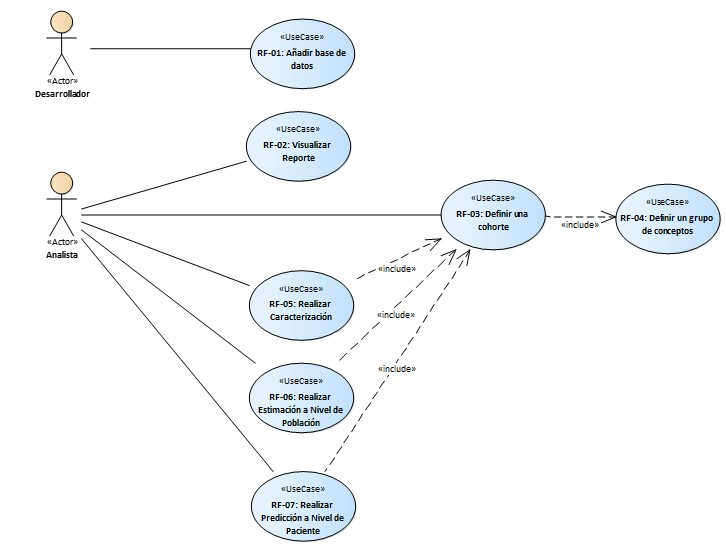
\includegraphics[width=0.90\textwidth]{figures/FRdiagram.jpg}
    \caption{Diagrama de casos de uso}
    \label{fig:FRdiagram}
\end{figure}

\subsection{Casos de uso del sistema} \label{subsec:06casosUso}

A continuación se detalla un diagrama de actividad y una tabla descriptiva para caso de uso presentado en la anterior Figura \ref{fig:FRdiagram} ''Diagrama de casos de uso''

\begin{figure}[H]
    \centering
    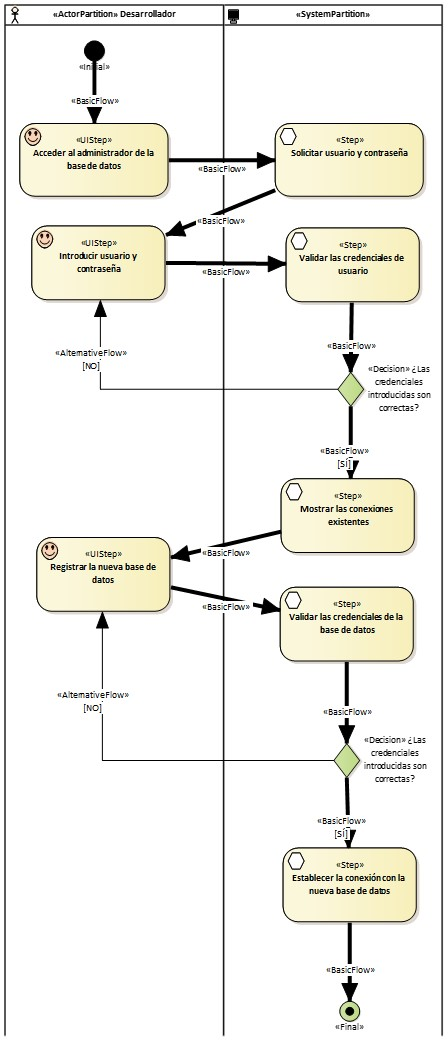
\includegraphics[width=0.60\textwidth]{figures/FR01.jpg}
    \caption{Diagrama de actividad de RF-01:Añadir base de datos}
    \label{fig:FR01}
\end{figure}

\begin{figure}[H]
    \centering
    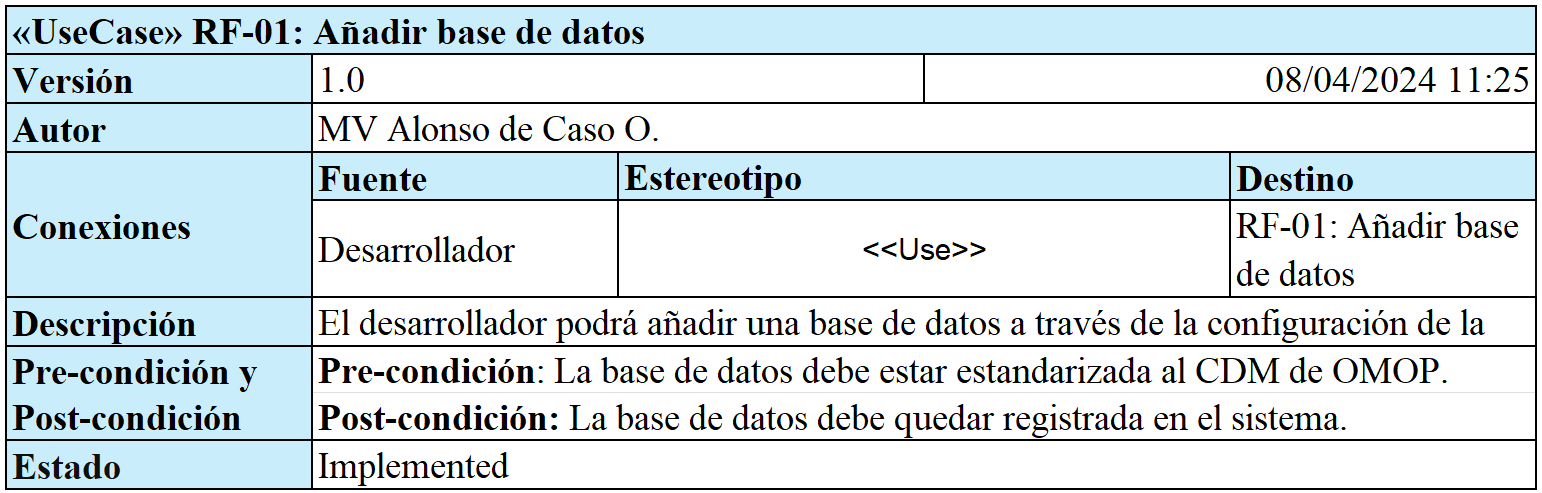
\includegraphics[width=0.80\textwidth]{tables/RF01tab.png}
    \captionof{table}{Caso de uso de RF-01:Añadir base de datos}
    \label{table:RF01tab}
\end{figure}

\begin{figure}[H]
    \centering
    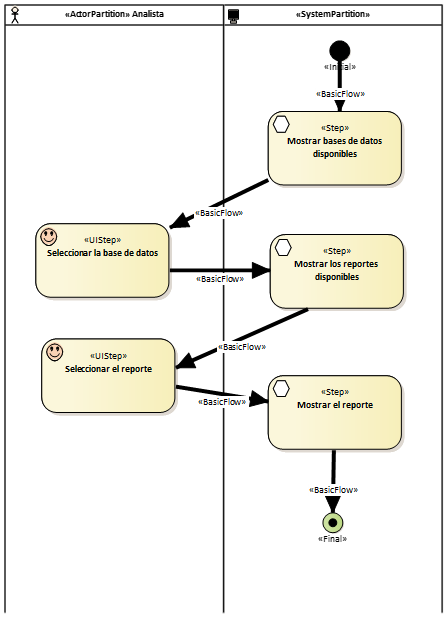
\includegraphics[width=0.65\textwidth]{figures/FR02.png}
    \caption{Diagrama de actividad de RF-02: Visualizar Reporte}
    \label{fig:FR02}
\end{figure}

\begin{figure}[H]
    \centering
    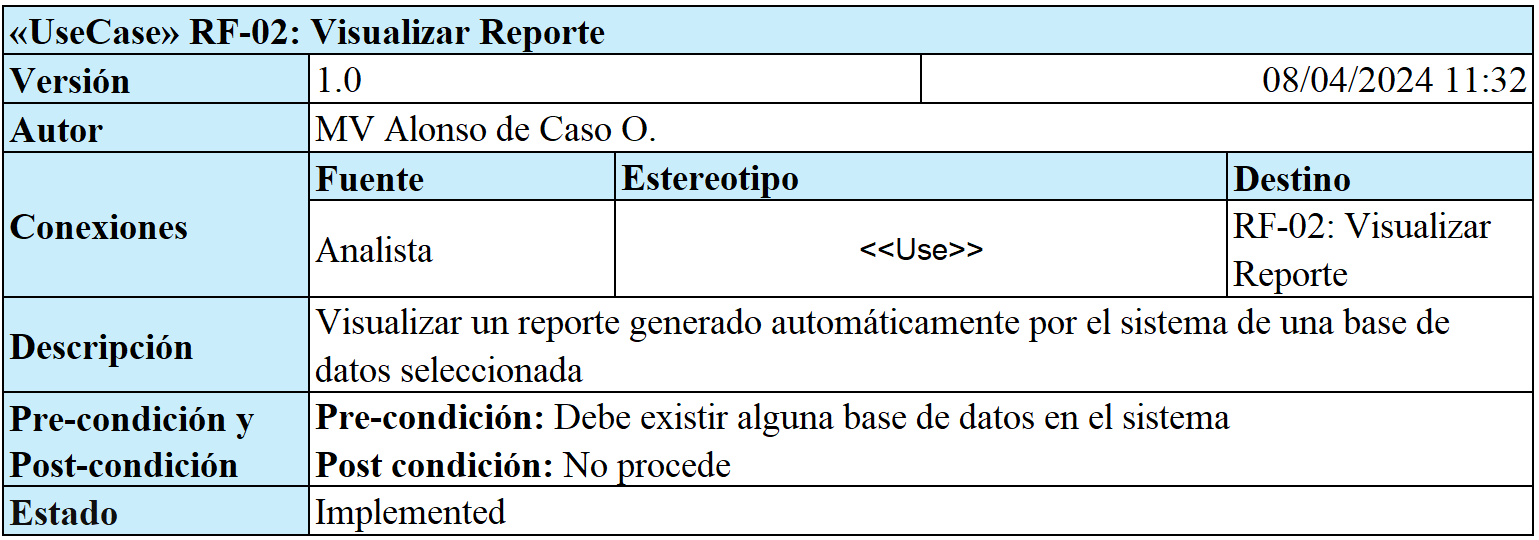
\includegraphics[width=0.80\textwidth]{tables/RF02tab.png}
    \captionof{table}{Caso de uso de RF-02:Visualizar Reporte}
    \label{table:RF02tab}
\end{figure}

\begin{figure}[H]
    \centering
    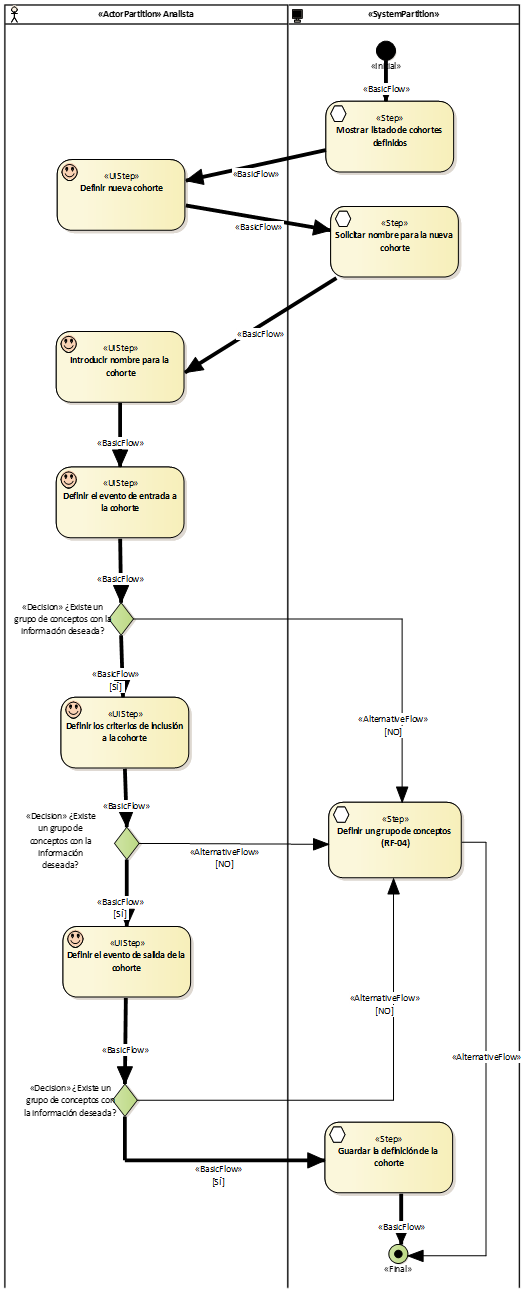
\includegraphics[width=0.60\textwidth]{figures/FR03.png}
    \caption{Diagrama de actividad de RF-03: Definir una cohorte}
    \label{fig:FR03}
\end{figure}

\begin{figure}[H]
    \centering
    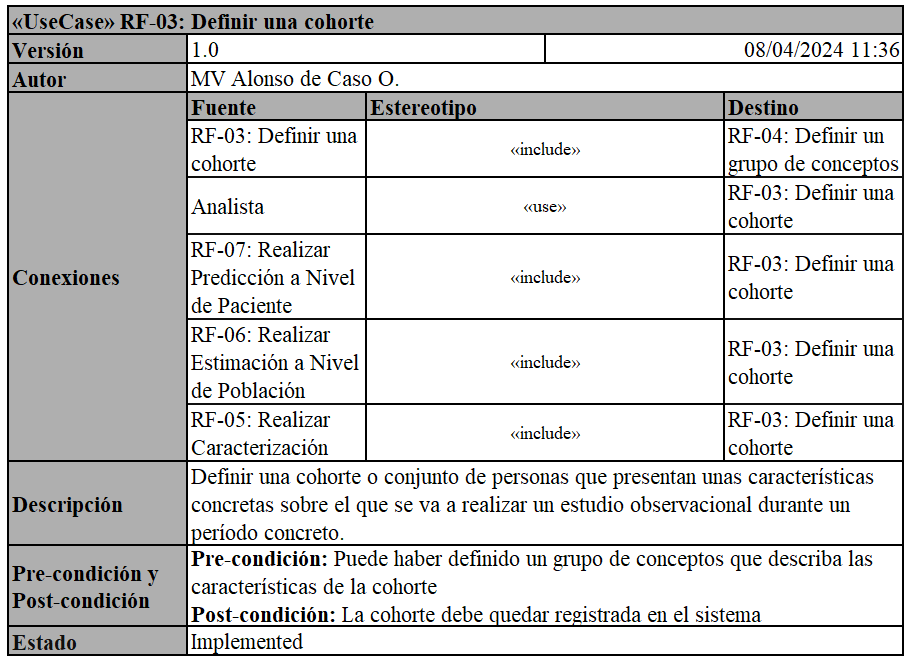
\includegraphics[width=0.80\textwidth]{tables/RF03tab.png}
    \captionof{table}{Caso de uso de RF-03:Definir una cohorte}
    \label{table:RF03tab}
\end{figure}

\begin{figure}[H]
    \centering
    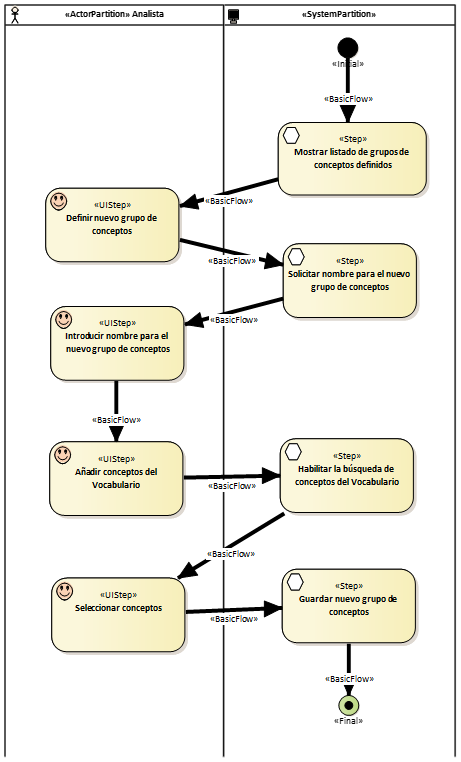
\includegraphics[width=0.65\textwidth]{figures/FR04.png}
    \caption{Diagrama de actividad de RF-04: Definir un grupo de conceptos}
    \label{fig:FR04}
\end{figure}

\begin{figure}[H]
    \centering
    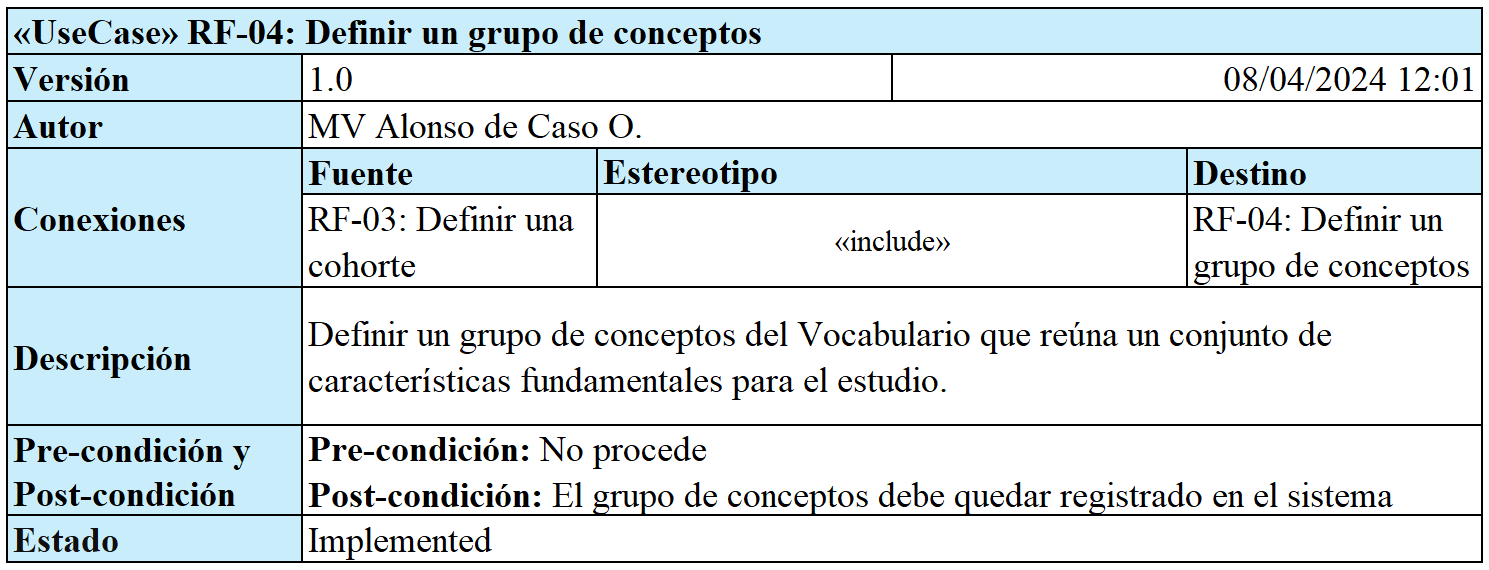
\includegraphics[width=0.80\textwidth]{tables/RF04tab.png}
    \captionof{table}{Caso de uso de RF-04:Definir un grupo de conceptos}
    \label{table:RF04tab}
\end{figure}

\begin{figure}[H]
    \centering
    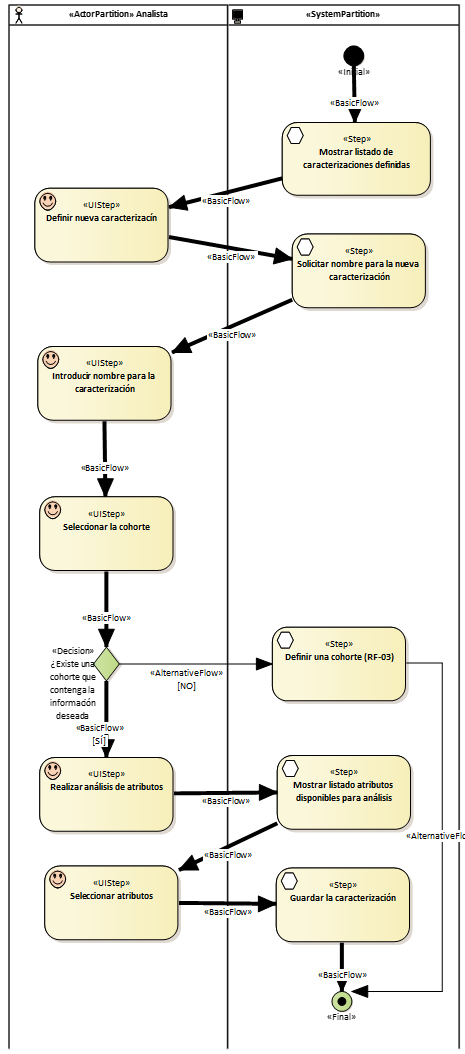
\includegraphics[width=0.65\textwidth]{figures/FR05.png}
    \caption{Diagrama de actividad de RF-05: Realizar Caracterización}
    \label{fig:FR05}
\end{figure}

\begin{figure}[H]
    \centering
    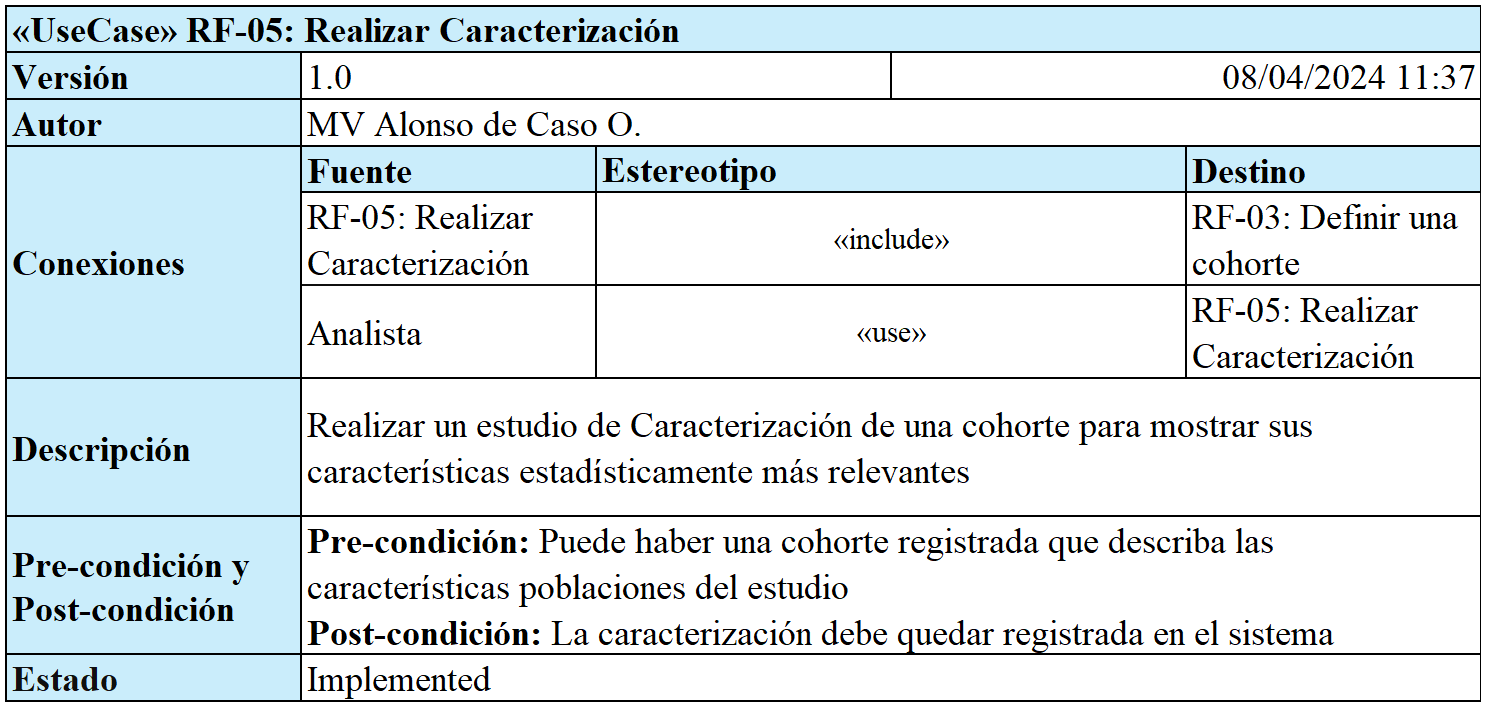
\includegraphics[width=0.80\textwidth]{tables/RF05tab.png}
    \captionof{table}{Caso de uso de RF-05: Realizar caracterización}
    \label{table:RF05tab}
\end{figure}

\begin{figure}[H]
    \centering
    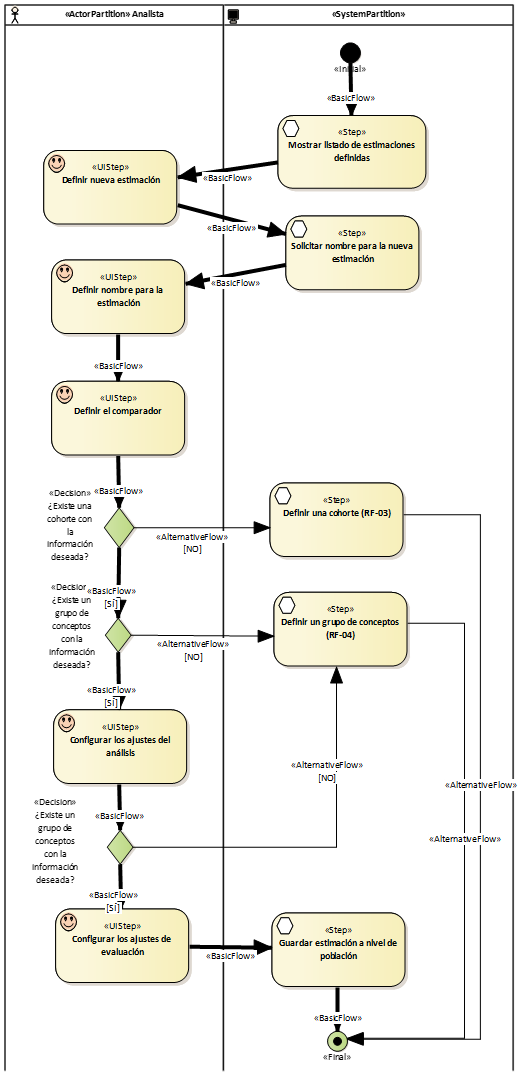
\includegraphics[width=0.65\textwidth]{figures/FR06.png}
    \caption{Diagrama de actividad de RF-06: Realizar caracterización}
    \label{fig:FR06}
\end{figure}

\begin{figure}[H]
    \centering
    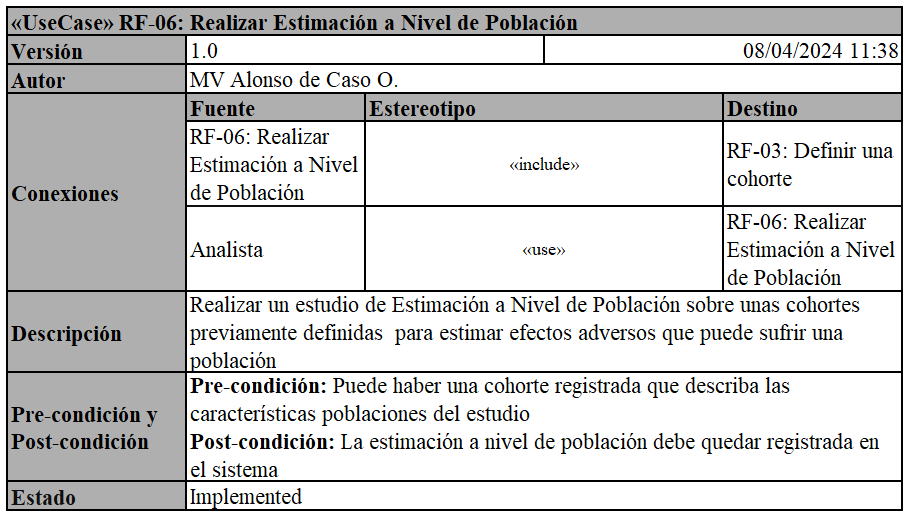
\includegraphics[width=0.80\textwidth]{tables/RF06tab.png}
    \captionof{table}{Caso de uso de RF-06: Realizar Estimación a nivel de Población }
    \label{table:RF06tab}
\end{figure}

\begin{figure}[H]
    \centering
    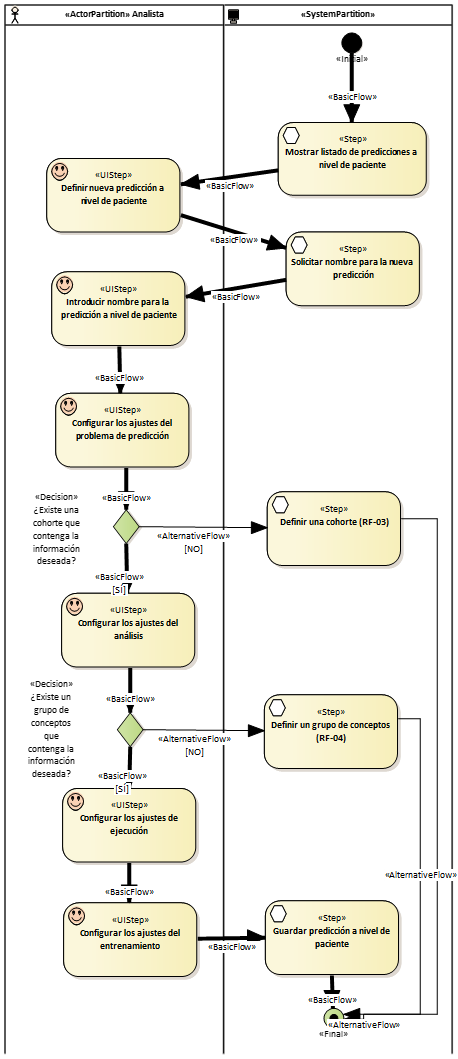
\includegraphics[width=0.80\textwidth]{figures/FR07.png}
    \caption{Diagrama de actividad de RF-07: Realizar Predicción a nivel de Paciente}
    \label{fig:FR07}
\end{figure}

\begin{figure}[H]
    \centering
    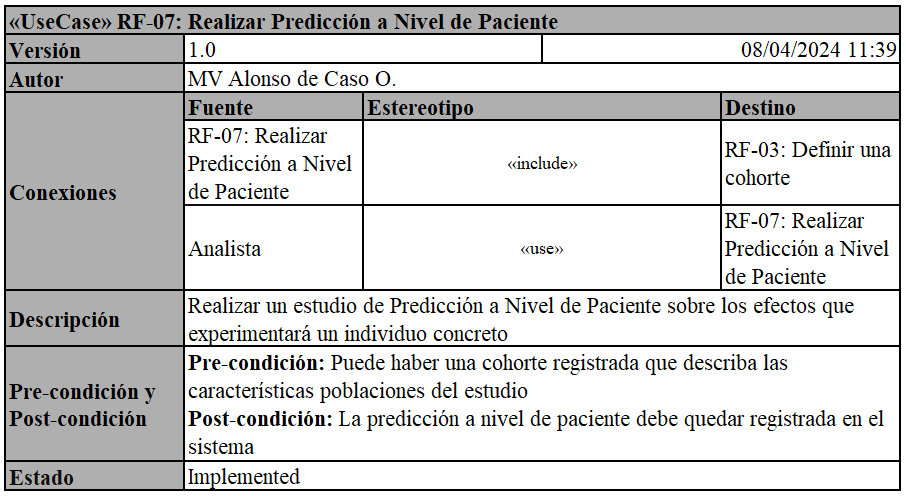
\includegraphics[width=0.80\textwidth]{tables/RF07tab.png}
    \captionof{table}{Caso de uso de RF-07: Realizar Predicción a nivel de Paciente }
    \label{table:RF07tab}
\end{figure}


\section{Requisitos no funcionales} \label{sec:06rnf}

Los requisitos no funcionales son restricciones o criterios de calidad que definen cómo debe comportarse un sistema, sin describir funciones específicas.

En base a lo aprendido sobre las características del sistema de ATLAS Broadsea, se han definido seis requisitos no funcionales.

A continuación se muestran estos requisitos de forma general en la Figura \ref{fig:RNFdiagram} ''Diagrama de requisitos no funcionales'' y posteriormente, se añade una tabla descriptiva para cada uno. 

\begin{figure}[H]
    \centering
    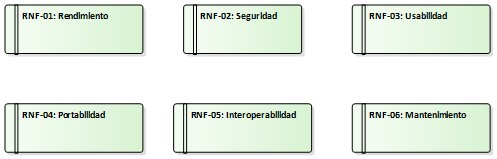
\includegraphics[width=0.90\textwidth]{figures/RNFdiagram.jpg}
    \caption{Diagrama de requisitos no funcionales}
    \label{fig:RNFdiagram}
\end{figure}

\begin{figure}[H]
    \centering
    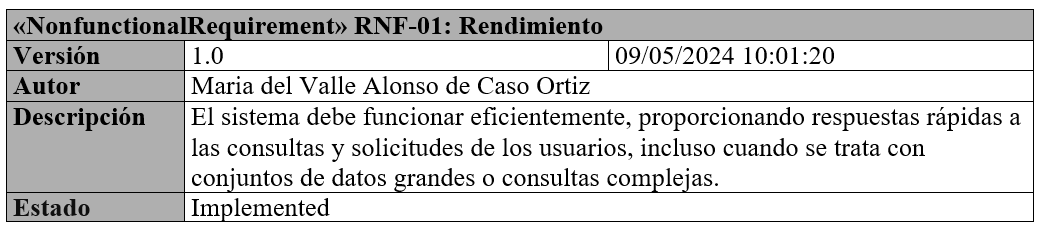
\includegraphics[width=0.90\textwidth]{tables/RNF01.png}
    \captionof{table}{RNF-01: Rendimiento}
    \label{fig:RNF01}
\end{figure}

\begin{figure}[H]
    \centering
    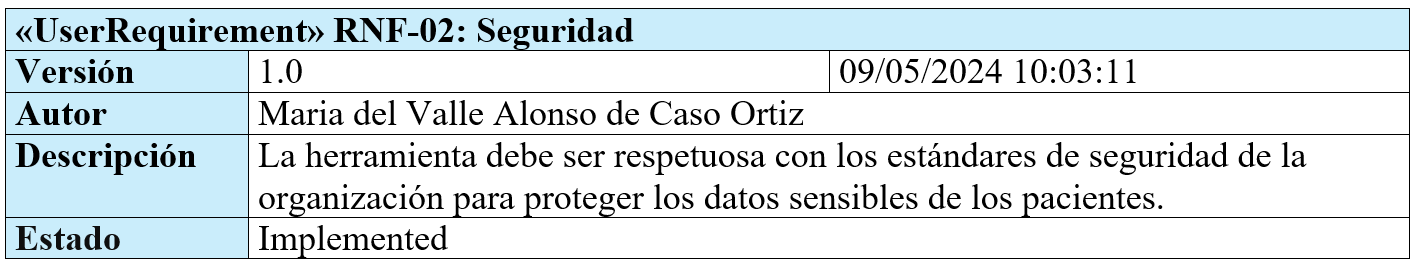
\includegraphics[width=0.90\textwidth]{tables/RNF02.png}
    \captionof{table}{RNF-02: Seguridad }
    \label{fig:RNF02}
\end{figure}

\begin{figure}[H]
    \centering
    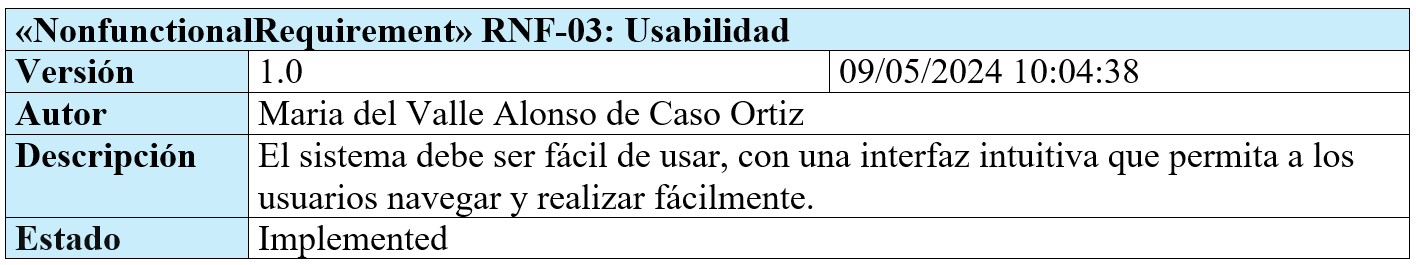
\includegraphics[width=0.90\textwidth]{tables/RNF03.png}
    \captionof{table}{RNF-03: Usabilidad }
    \label{fig:RNF03}
\end{figure}

\begin{figure}[H]
    \centering
    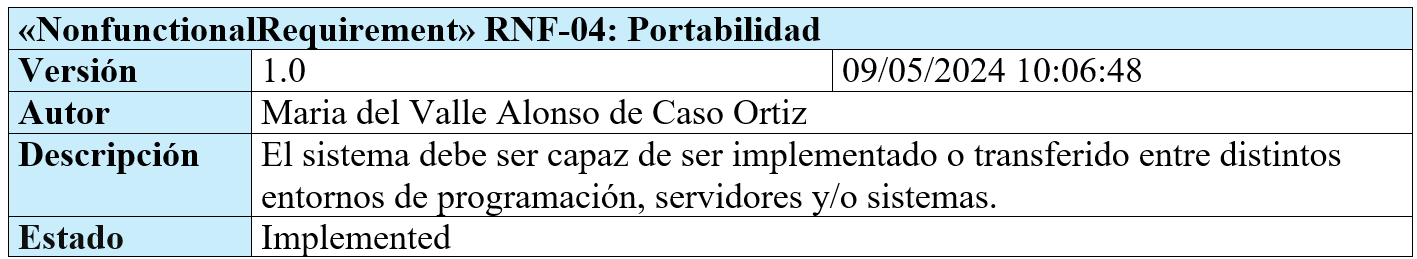
\includegraphics[width=0.90\textwidth]{tables/RNF04.png}
    \captionof{table}{RNF-04: Portabilidad}
    \label{fig:RNF04}
\end{figure}

\begin{figure}[H]
    \centering
    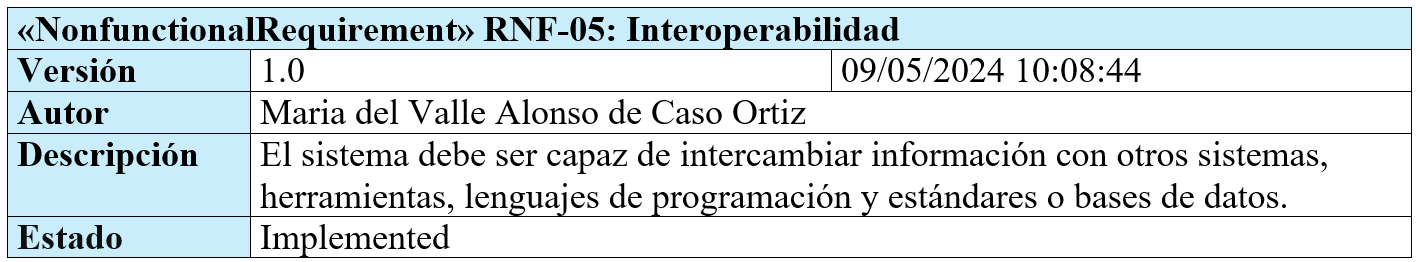
\includegraphics[width=0.90\textwidth]{tables/RNF05.png}
    \captionof{table}{RNF-05: Interoperabilidad}
    \label{fig:RNF05}
\end{figure}

\begin{figure}[H]
    \centering
    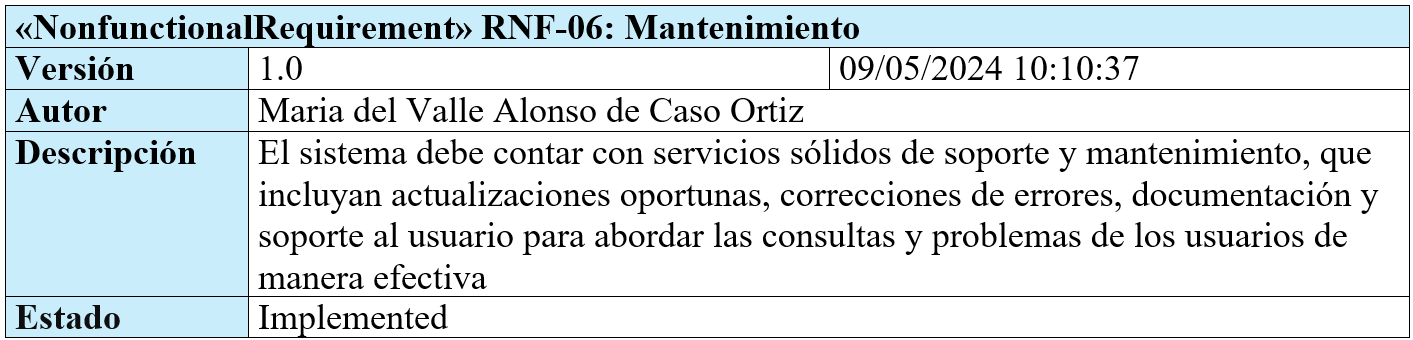
\includegraphics[width=0.90\textwidth]{tables/RNF06.png}
    \captionof{table}{RNF-06: Mantenimiento}
    \label{fig:RNF06}
\end{figure}

\section{Conclusiones} \label{sec:06conclusiones}

De este capítulo se concluye que, aunque el objetivo del proyecto no sea específicamente diseñar un sistema, el análisis de requisitos es de gran relevancia y utilidad  para esquematizar y comprender las funcionalidades del sistema y sus propiedades.

Gracias a este análisis se abstrae de forma más sencilla el funcionamiento y las tareas que realiza el sistema de Broadsea, que en realidad es bastante más complejo.
